\documentclass[pdf, unicode, 12pt, a4paper,oneside,fleqn]{article}

\usepackage{styles/log-style}
\begin{document}

\begin{titlepage}
\begin{center}
\bfseries
{\Large Московский авиационный институт\\ (национальный исследовательский университет)}

\vspace{48pt}
{\large Факультет информационных технологий и прикладной математики}

\vspace{36pt}
{\large Кафедра вычислительной математики и программирования}

\vspace{48pt}Лабораторная работа \textnumero 4 по курсу 
\enquote{Численные методы}
\end{center}
\vspace{72pt}

\begin{flushright}
\begin{tabular}{rl}
Студент: & П.\,А. Гамов \\
Преподаватель: & Д.\,Л. Ревизников \\
Группа: & М8О-407Б \\
Дата: & \\
Оценка: & \\
Подпись: & \\
\end{tabular}
\end{flushright}
\vfill
\begin{center}
\bfseries
Москва, \the\year
\end{center}
\end{titlepage}

\pagebreak

\section{Численные методы решения обыкновенных дифференциальных уравнений}

\subsection{Метод Эйлера}

\begin{lstlisting}
def euler_method(x, y0, z0, h, f = f_xyz):
    y, z = [y0], [z0]
    for k in range(len(x) - 1):
        y.append(y[k] + h*z[k])
        z.append(z[k] + h*f(x[k], y[k], z[k]))
    return y, z
\end{lstlisting}


Точное решение:

2.649 2.574 2.545 2.560 2.617 2.720 2.873 3.083 3.363 3.726 4.195 

Решение явным методом Эйлера:

2.649 2.549 2.502 2.500 2.541 2.624 2.751 2.927 3.158 3.454 3.828 

Точное значение первой производной:

-1.000 -0.509 -0.067 0.359 0.795 1.267 1.801 2.428 3.185 4.119 5.292 

Значение первой производной решения явным методом Эйлера:

-1.000 -0.470 -0.014 0.410 0.829 1.270 1.755 2.309 2.959 3.741 4.696 

Погрешность решения: 0.5582367523703139

Погрешность производной: 0.7574105372312112

Погрешность решения: 0.25935785742625495

Погрешность производной: 0.3321641637820709

\subsection{Метод Эйлера-Коши}

\begin{lstlisting}
def euler_cauchy_method(x, y0, z0, h, f = f_xyz):
    y = [y0]
    z = [z0]
    for k in range(len(x) - 1):
        yk = y[k] + h*z[k]
        zk = z[k] + h*f(x[k], y[k], z[k])
        y.append(y[k] + h*(z[k] + zk) / 2)
        z.append(z[k] + h*(f(x[k], y[k], z[k]) + f(x[k+1], yk, zk)) / 2)
    return y, z
\end{lstlisting}

Решение явным методом Эйлера-Коши:

2.649 2.575 2.548 2.563 2.620 2.723 2.875 3.085 3.362 3.723 4.186 

Погрешность решения: 0.010673398095964622

Погрешность производной: 0.015331681582464311

Погрешность решения: 0.0025520103059432776

Погрешность производной: 0.0037731392264878766

\subsection{Метод Рунге-Кутты 4-го порядка}

\begin{lstlisting}
def delta(xk, yk, zk, h, f):
    K1 = h * zk
    L1 = h * f(xk, yk, zk)
    K2 = h * (zk + L1 / 2)
    L2 = h * f(xk + h/2, yk + K1/2, zk + L1/2)
    K3 = h * (zk + L2 / 2)
    L3 = h * f(xk + h/2, yk + K2/2, zk + L2/2)
    K4 = h * (zk + L3)
    L4 = h * f(xk + h, yk + K3, zk + L3)
    return ((K1 + 2*K2 + 2*K3 + K4)/6, (L1 + 2*L2 + 2*L3 + L4)/6)

def runge_kutta_metod(x, y0, z0, h, f = f_xyz):
    y = [y0]
    z = [z0]
    for k in range(len(x) - 1):
        delta_ = delta(x[k], y[k], z[k], h, f)
        y.append(y[k] + delta_[0])
        z.append(z[k] + delta_[1])
    return y, z
\end{lstlisting}

Решение методом Рунге-Кутты 4-го порядка:

2.649 2.574 2.545 2.560 2.617 2.720 2.873 3.083 3.363 3.726 4.195 

Значение первой производной решения методом Рунге-Кутты:

-1.000 -0.509 -0.067 0.359 0.795 1.267 1.801 2.428 3.185 4.119 5.292 

Погрешность решения: 2.243362412801516e-05

Погрешность производной: 3.358057253144096e-05

Погрешность решения: 1.4035550461825057e-06

Погрешность производной: 2.1052860420152156e-06

\subsection{Метод Адамса}

\begin{lstlisting}
def adams_z(x, y, z, h, f, k):
    return z[k] + h*(
        55*f(x[k], y[k], z[k]) -
        59*f(x[k-1], y[k-1], z[k-1]) +
        37*f(x[k-2], y[k-2], z[k-2]) -
        9*f(x[k-3], y[k-3], z[k-3])) / 24

def adams_y(x, y, z, h, f, k):
    return y[k] + h*(55*z[k] - 59*z[k-1] + 37*z[k-2] - 9*z[k-3]) / 24

def adams_method(x, y0, z0, h, f = f_xyz):
    y, z =  runge_kutta_metod(x[:4], y0, z0, h, f)
    for k in range(3, len(x)-1):
        y.append(adams_y(x, y, z, h, f, k))
        z.append(adams_z(x, y, z, h, f, k))
    return y, z
\end{lstlisting}

Решение методом Адамса в узлах сетки:

2.649 2.574 2.545 2.560 2.618 2.720 2.872 3.082 3.361 3.723 4.189 

Значение первой производной решения методом Адамса:

-1.000 -0.509 -0.067 0.359 0.793 1.264 1.797 2.422 3.177 4.108 5.276 

Погрешность решения: 0.0065999421014504185

Погрешность производной: 0.022317754207798305

Погрешность решения: 0.0003900960620764228

Погрешность производной: 0.0013372594756700053

\subsection{График функции}

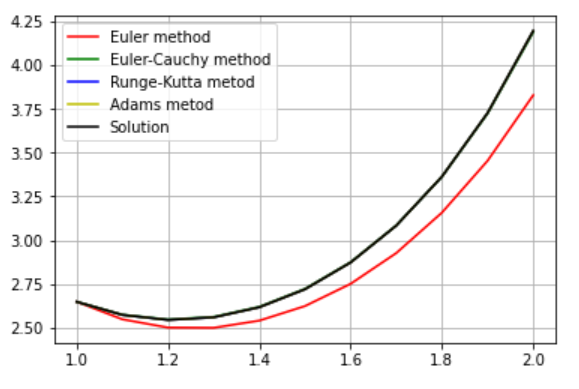
\includegraphics[scale=0.45]{data1.png}

\subsection{График производной}

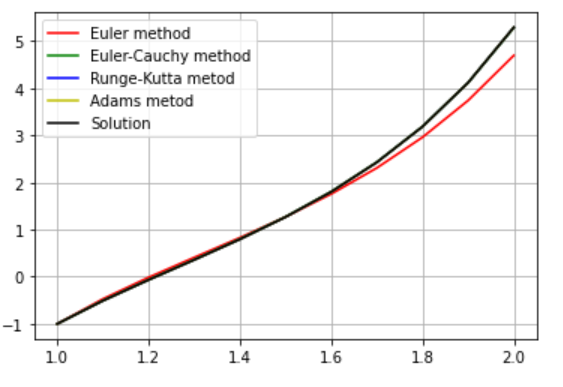
\includegraphics[scale=0.45]{data2.png}

\subsection{Логарифмическая ошибка}

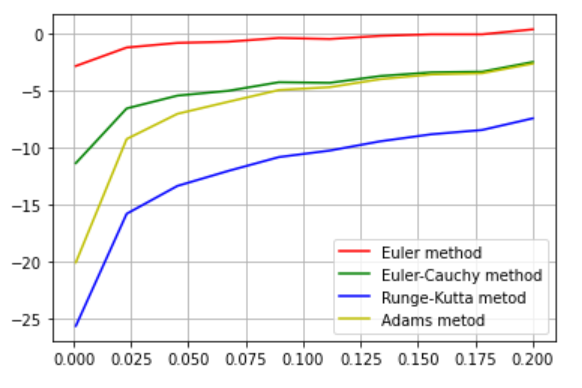
\includegraphics[scale=0.45]{data3.png}

\section{Численные методы решения обыкновенных дифференциальных уравнений}

\subsection{Mетод рунге-кутты}

\begin{lstlisting}
def delta(xk, yk, zk, h, f):
    K1 = h * zk
    L1 = h * f(xk, yk, zk)
    K2 = h * (zk + L1 / 2)
    L2 = h * f(xk + h/2, yk + K1/2, zk + L1/2)
    K3 = h * (zk + L2 / 2)
    L3 = h * f(xk + h/2, yk + K2/2, zk + L2/2)
    K4 = h * (zk + L3)
    L4 = h * f(xk + h, yk + K3, zk + L3)
    return ((K1 + 2*K2 + 2*K3 + K4)/6, (L1 + 2*L2 + 2*L3 + L4)/6)
    
def runge_kutta_method(x, y0, z0, h, f = f_xyz):
    y = [y0]
    z = [z0]
    for k in range(len(x) - 1):
        delta_ = delta(x[k], y[k], z[k], h, f)
        y.append(y[k] + delta_[0])
        z.append(z[k] + delta_[1])
    return y
\end{lstlisting}

\subsection{Метод стрельбы}

\begin{lstlisting}
def shooting_method(x, y0, y1, h, f = f_xyz, e = 0.00001):
    et_prev = 1
    et_i = 0.8
    y_prev = runge_kutta_method(x, y0, et_prev, h, f)
    y_i = runge_kutta_method(x, y0, et_i, h, f)
    Fi_prev = y_prev[-1] - y1
    Fi_i = y_i[-1] - y1
    while abs(Fi_i) > e:
        et_prev, et_i = et_i, et_i - Fi_i * (et_i - et_prev) / (Fi_i - Fi_prev)
        y_prev, y_i = y_i, runge_kutta_method(x, y0, et_i, h, f)
        Fi_prev, Fi_i = Fi_i, y_i[-1] - y1
    return y_i
\end{lstlisting}

Метод стрельбы:

3.773 3.651 3.558 3.486 3.430 3.388 3.355 3.332 3.314 3.303 3.296 

Точность: 5.396833470110098e-06

Рунге-Ромберг: 1.7030199027697287e-12

\subsection{Конечно-разностный метод}

\begin{lstlisting}
def finite_differences_method(x, y0, y1, h, p = p_x, q = q_x, f = f_x):
    A = find_tridig_A(h, p, q, x)
    b = find_b(h, p, f, x, y0, y1)
    y = [y0] + tridig_matrix_alg(A, b) + [y1]
    return y
def find_b(h, p, f, x, y0, y1):
    b = [h*h*f(x[i]) for i in range(1, len(x[:-1]))]
    b[0] -= y0*(1 - p(x[1])*h/2)
    b[-1] -= y1*(1 + p(x[-2])*h/2)
    return b
def find_tridig_A(h, p, q, x):
    A = [[1 - (p(x[i]))/2, (-2 + h*h*q(x[i])), 1 + (p(x[i])*h)/2] for i in range(1, len(x[:-1]))]
    A[0][0] = 0
    A[-1][-1] = 0
    return A
def tridig_matrix_alg(A, b):
    P = [-item[2] for item in A]
    Q = [item for item in b]
    P[0] /= A[0][1]
    Q[0] /= A[0][1]
    for i in range(1, len(b)):
        z = (A[i][1] + A[i][0] * P[i-1])
        P[i] /= z
        Q[i] -= A[i][0] * Q[i-1]
        Q[i] /= z
    x = [item for item in Q]
    for i in range(len(x) - 2, -1, -1):
        x[i] += P[i] * x[i + 1]
    return x
\end{lstlisting}

Конечно-разностный метод:

3.773 3.652 3.558 3.487 3.431 3.388 3.356 3.332 3.315 3.303 3.296 

Точность: 0.0020476449984153534

Рунге-Ромберг: 1.5649567837103733e-07

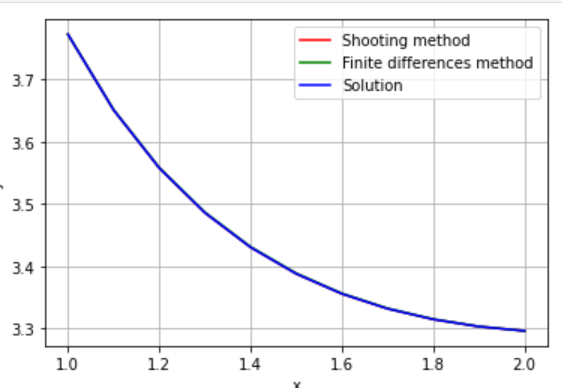
\includegraphics[scale=0.45]{data4.png}

\section{Выводы}

В данной лабораторной работе я научился решать численно дифференциальные уравнения второго порядка.

\end{document}